




\begin{figure}[!t]
    \centering
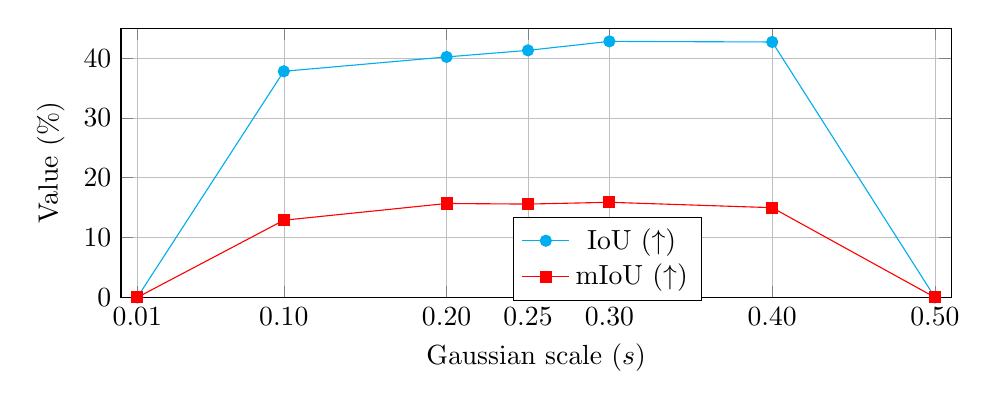
\begin{tikzpicture}
    \begin{axis}[
        width=\columnwidth, %
        height=5cm, %
        xlabel={Gaussian scale ($s$)},
        ylabel={Value (\%)},
        xmin=0, xmax=0.51,
        ymin=0, ymax=45,
        xtick={0.01, 0.10, 0.20, 0.25, 0.30, 0.40, 0.50},
        xticklabels={0.01, 0.10, 0.20, 0.25, 0.30, 0.40, 0.50},
        ytick={0, 10, 20, 30, 40}, %
        legend style={at={(0.7, 0.3)}}, %
        grid=both,
        grid style={line width=.1pt, draw=gray!10},
        major grid style={line width=.2pt, draw=gray!50},
    ]
        \addplot[
            color=cyan,
            mark=*,
            mark options={solid, fill=cyan},
        ] coordinates {
            (0.01, 0.0)
            (0.10, 37.8)
            (0.20, 40.2)
            (0.25, 41.3)
            (0.30, 42.8)
            (0.40, 42.7)
            (0.50, 0.0)
        };
        \addlegendentry{IoU ($\uparrow$)}

        \addplot[
            color=red,
            mark=square*,
            mark options={solid, fill=red},
        ] coordinates {
            (0.01, 0.0)
            (0.10, 12.9)
            (0.20, 15.7)
            (0.25, 15.6)
            (0.30, 15.9)
            (0.40, 15.0)
            (0.50, 0.0)
        };
        \addlegendentry{mIoU ($\uparrow$)}
    \end{axis}
\end{tikzpicture}
    \caption{\textbf{Impact of fixed Gaussian scales on 3D mIoU and IoU} using TPVFormer \cite{huang2023tpv} trained using only $L_{\text{2D}}$ without $L_{\text{3D}}$ on 20\% of Occ3d-nuScenes \cite{tian2023occ3d} validation dataset.}
    \label{fig:impact_of_scale}
\end{figure}
